%% LaTeX2e class for student theses
%% sections/evaluation.tex
%% 
%% Karlsruhe Institute of Technology
%% Institute of Information Security and Dependability
%% Software Design and Quality (SDQ)
%%
%% Dr.-Ing. Erik Burger
%% burger@kit.edu
%%
%% Version 1.6, 2024-06-07

\chapter{Evaluation}
\label{ch:Evaluation}
The purpose of the evaluation of the implemented prototype is to empirically assess the capabilities of the developed approach to pattern matching of TGG rules on atomic model changes.

Therefore, one concern is to determine the automatization degree in terms of consistency completeness, i.e., the expressiveness for consistency conditions, the rule representation complexity (the avoidance of data loss) and performance of TGG usage on available \textsc{Vitruvius} evaluation cases like those used in the article describing the \textsc{Vitruvius} approach \cite{VitruviusKlare2021} and based on that compare them with preexisting consistency preservation languages.
To that end, the evaluation cases were extended, translating existing rules to TGG rules wherever possible.

A second concern, that of scalability, was evaluated by randomly generating models from the TGG rules in the evaluation case \emph{HospitalToAdministration}, which is from the emoflon::IBeX tutorial \cite{emoflon_tutorial, noauthor_github_emoflon_tutorial}.
The idea is to generate models of various sizes and measure the asymptotical runtime performance of the prototype.

\section{GQM Plan}
\label{sec:Evaluation:GQMPlan}
The evaluation is structured by following a Goal Question Metric (GQM) plan, as proposed by Basili et al. \cite{basili_methodology_gqm_1984}, to enable transparent methodical verifiability and to explicitly consider construct validity.

\begin{gqm}
    \item Ensuring correctness of the consistency preservation process
    \begin{gqm}
        \item Does the approach identify complex changes correctly?
        \begin{gqm}
            \item Number of change sequences that are incorrectly matched
        \end{gqm}
    \end{gqm}
    \item Preserving consistency completeness
    \begin{gqm}
        \item Can realistic consistency relations be represented by the TGG approach?
        \begin{gqm}
            \item Number of rules that can be represented by TGG rules.
        \end{gqm}
    \end{gqm}
    \item Preserving or improving performance of consistency preservation
    \begin{gqm}
        % \item How does the TGG approach perform in comparison to existing approaches in (semi-) realistic scenarios
        % \begin{gqm}
        %     \item Runtime of consistency preservation algorithm on change sequences
        % \end{gqm}
        \item How does the approach perform in comparison to existing approaches?
        \begin{gqm}
            \item Runtime trend of consistency preservation algorithm on change sequences in dependence of input nodes and change sequence length.
            \item Runtime trend of different subroutines of the consistency preservation algorithm on change sequences in dependence of input nodes and change sequence length.
        \end{gqm}
    \end{gqm}
\end{gqm}

In \autoref{sec:Evaluation:Design}, the realization of the GQM plan are explained in full detail.
Section \ref{sec:Evaluation:Results} presents and discusses the results of the evaluation according to the method described in \autoref{sec:Evaluation:Design}.

\section{Method}
\label{sec:Evaluation:Design}
In this section, the general preconditions for conducting the evaluation are described. This includes the used evaluation cases and the procedure.
Then, each goal described in the GQM Plan (see \autoref{sec:Evaluation:GQMPlan}) and their respective setup constellations are explained.

\paragraph{Evaluation Cases} In the preparation of this evaluation, two evaluation cases were chosen for the accomplishment of the three goals to depend on:
\begin{itemize}
    \item \textbf{G1}, \textbf{G2}: \emph{JavaToUml} \cite{noauthor_vitruv-toolsvitruv-casestudies_nodate, chen_java-to-uml} 
    \item \textbf{G3}: \emph{HospitalToAdministration} \cite{emoflon_tutorial, noauthor_github_emoflon_tutorial}
\end{itemize}

In the case of \emph{JavaToUml}, existing consistency preservation rules, written in the reactions language \cite{kramer_specification_2017}, were attempted to translate into TGG rules by hand.
% \todo{JavaToUml detaillierter beschreiben, Metamodelle und bestehende reactions}

\subsection{G1 - Ensuring correctness of the consistency preservation process}
\label{sec:Evaluation:Design:G1}
Ensuring correctness of the consistency preservation process is the first goal of the evaluation of the prototype.
The TGG rules written for the two evaluation cases form the basis for being able to reach that goal.
The following question is answered:

\paragraph{Q1.1} Does the approach identify complex changes correctly?\newline
To answer that question, we define a number of change sequences so that each TGG rule is covered at least once.
We further define which matches are expected for each change sequence.
Based on that, the number of change sequences whose matches deviates from the expectation, and are thus \emph{incorrectly matched}, is determined.
Further, that same number of incorrectly matched patterns under the fiction of not having the proxy problem described in \autoref{sec:Implementation:Challenges:unsolved} is determined. Due to the fictional nature, this is done by comparing the change sequences that are incorrectly matched due to the proxy problem to other change sequences that don't fall under the proxy problem and assuming that they would behave in the same way. For each of those, a \enquote{partner rule} is determined to make this metric more traceable and replicable.

Since the outcome of that metric and its proxy-problem ignoring counterpart depends on how change sequences are chosen, their choice is oriented towards the evaluation case.

% This way, the first metric indicates how often incorrectly matched patterns occur and the second metric indicates how many rules can be expected to be \enquote{safe to use}.


\subsection{G2 - Preserving consistency completeness}
\label{sec:Evaluation:Design:G2}
To evaluate to what extend the goal of preserving consistency completeness is reached, the following question is answered:

\paragraph{Q2.1} Can realistic consistency relations be represented by the TGG approach? \newline
The choice of using the evaluation case \emph{JavaToUml} for the evaluation roots in this question. Both Java and UML are non-artificial metamodels which have been modeled in the Eclipse Modeling Framewok. Since there are overlaps in the concepts that both metamodels describe, consistency relations between both metamodels can be deemed realistic and have also been modeled in the \emph{Reactions} language \cite{kramer_specification_2017} prior to this thesis.
To answer the question, that \emph{consistency preservation rules} (CPRs), represented by reactions, are looked upon. 
The effects of each reaction are tried to be modeled with TGG rules that are processable in the prototype.
Then, each rule is categorized into one of the following categories:
\begin{itemize}
    \item \emph{Full preservation}: The consistency preservation rule is equivalently implemented by both the reaction and the TGG rule(s).
    \item \emph{Partial preservation}: The consistency preservation rule expressed by the reaction can only be implemented partially by TGG rules. Some aspects are implementable and processable, some are not.
    \item \emph{No preservation} The consistency preservation rule can not be expressed with TGG rules or not be processed by the prototype
\end{itemize}
For each category, the number of CPRs that fall into that category is determined. For partial or no preservation, reasons are given.


\subsection{G3 - Preserving or improving performance of consistency preservation}
\label{sec:Evaluation:Design:G3}
Having set the goal of preserving or improving performance of consistency preservation with the concept, the following question is to be answered:

\paragraph{Q3.1} How does the approach perform in comparison to existing approaches? \newline
The question of performance and scalability rises as using preexistent information on the actual changes to generate matches is an approach in which the search space is smaller and thus, it can be hypothesized that less computing time is needed to find rule matches and propagate them to the target model.
However, since the concept and prototype include a selection of pattern matches (see \autoref{sec:Concept:PatternSelection}), this must be taken into account when comparing the approach to another pattern matcher that does not perform this.
The other pattern matcher is the \emph{high-performance pattern matcher} \textsc{HiPE} \cite{hipe-devops_highly_2022} included in the eMoflon::IBeX framework.
For easier referencing, the approach in this thesis is called \textsc{VitruvTGG} in the context of evaluation.
The following time measurements are taken:
\begin{itemize}
    \item \textsc{VitruvTGG}: 
        \begin{itemize}
            \item Main green forward matching time: The time spent for the green matching of the change sequence against the ChangeSequenceTemplates
            \item Total context matching time: The cumulated time spent on trying to match context for green matches that have not yet been applied.
            \item Total coverage flattening time: The cumulated time spent on \emph{coverage flattening}, i.e. ensuring that each change is covered by at most one match.
            \item Total change propagation time: The total runtime of the change propagation
        \end{itemize}
    \item \textsc{HiPE}: Total change propagation time: The total runtime of the change propagation
\end{itemize}

\paragraph{Experimental Setup}
The experimental setup is designed in the following way:
Models, and thus change sequences, of different sizes are generated randomly with the eMoflon::IBeX \textsc{Modelgen} application. This application generates a \enquote{random} triple graph based on a TGG ruleset. \textsc{Modelgen} has limitations that restrict the choice of model size measure. While it is possible to specify a maximum amount of graph elements this cannot be the only constraint since \textsc{Modelgen} only applies one rule if only that constraint is given. To nudge \textsc{Modelgen} to more randomness, the max count of rules is also included, calculated as follows: $maxApplicationsPerRule=graphElementSize / numberOfRules$.
Although a rule application always creates at least one graph element, These further constraints have repercussions on the resulting graph element size, because situations might occur where some rules have reached their max count and all others are not applicable to the current situation anymore.
The procedure is as follows: For $graphElementSize = 2^3, 2^4, \dots, 2^{11}$, the following steps are taken with both the \textsc{HiPE} and the \textsc{VitruvTGG} pattern matcher:
\begin{enumerate}
    \item Generate triple graph with source element size $graphElementSize$ and the aforementioned additional constraints.
    \item Delete correspondences, protocol and target graph.
    \item Generate a change sequence from $\emptyset$ to $model$ using \textsc{Vitruvius} classes that use EMF Compare \cite{noauthor_emf_compare}.
    \item Start change propagation and measure the times described above.
    \item Repeat steps 1 to 4 with this parametrization $20$ times.
    \item calculate the median and store the results.
\end{enumerate}
That procedure is automated using \emph{JUnit 5} \cite{noauthor_junit_nodate}.
Performance measurements are executed on a machine with the following specifications:
\begin{itemize}
    \item Processor: Intel Core i9-8950HK
    \item Random Access Memory: $32.0$ GB, $2667$ MHz
    \item Operating System: Windows 10 Pro
\end{itemize}


% \paragraph{Q3.2} \todo{TODO EVENTUELL}: Check second approach: generate 2048-model and don't delete corr, source and target! Perform 8,16,32,64,128,256,512,... changes. Hypothesis: Here, Vitruv might perform bettern than in Q3.1 since the prototype  knows where the changes happened.
% The question of performance and scalability rises as using preexistent information on the actual changes to generate matches is an approach in which the search space is smaller
% \todo{schreibne}

\section{Results}
\label{sec:Evaluation:Results}
In this section, the results of the evaluation that was performed following the method in \autoref{sec:Evaluation:Design} are presented.

\subsection{G1 - Ensuring correctness of the consistency preservation process}
\label{sec:Evaluation:Results:G1}
In \autoref{tab:M1.1.1}, the results of evaluating the prototype on \emph{JavaToUML} with metric \emph{M1.1.1} can be seen.
It is noticeable, that while with $57.78\%$, the number of correctly matched patterns can be considerd relatively low, the number of correctly matched patterns if there was no proxy problem is relatively high ($95.56\%$).
That can be interpreted as a good sign for the correctness of the concept but a drawback for the prototype or the framework that introduces the proxy problem. 
\begin{table}[h!]
\centering
\begin{tabular}{c | c  c c c}
    \toprule
     &      & \multicolumn{3}{c}{matching categories} \\
            & total & \makecell{incorrectly \\ matched} & \makecell{correctly \\ matched} & \makecell{correctly matched \\ if there was no proxy problem}\\
    \midrule
    \makecell{Number of \\ change sequences}  & $45$ & $19$ & $26$ & $43$\\
    Proportion of total    & $100\%$ & $42.22\%$ & $57.78\%$ & $95.56\%$ \\
    % 789 & 0AB\\
    \bottomrule
\end{tabular}
\caption{Results of metric M1.1.1 on evaluation case JavaToUml}
\label{tab:M1.1.1}
\end{table}

\subsection{G2 - Preserving consistency completeness}
\label{sec:Evaluation:Results:G2}
In \autoref{tab:M2.1.1}, the results of evaluating the prototype on \emph{JavaToUML} with metric \emph{M2.1.1} can be seen.
With  $93.33\%$, consistency completeness can be interpreted as high, considering that the baseline is a turing-complete imperative language while the protoype's imperativity is limited to attribute conditions.

\begin{table}[h!]
% \centering\small
\centering
\begin{tabular}{c | c  c c c}
    \toprule
     &      & \multicolumn{3}{c}{representability} \\
            & total & full & partial & None \\
    \midrule
    Number of consistency preservation rules  & $45$ & $42$ & $2$ & $1$\\
    Proportion of total    & $100\%$ & $93.33\%$ & $4.44\%$ & $2.22\%$ \\
    % 789 & 0AB\\
    \bottomrule
\end{tabular}
\caption{Results of metric M2.1.1 on evaluation case JavaToUml}
\label{tab:M2.1.1}
\end{table}

The cases where the consistency preservation rules defined in the \emph{Reactions} langugage could not be fully represented and the reasons for that are discussed in the following.

Reactions that could only be partially reppresented with TGG rules include \newline\texttt{JavaCompilationUnitInsertedInPackage} and \texttt{JavaClassifierRemoved}.
\newline\texttt{JavaCompilationUnitInsertedInPackage}, as can be seen in \autoref{javaCompilationUnitInsertedInPackage} includes adding correspondences between the metamodel element \texttt{UMLPackage.Literals.PRIMITIVE\_TYPE} and model elements. This cannot be mapped with TGGs.


\begin{figure}
\centering
\begin{lstlisting}[language=java, caption={Reaction JavaCompilationUnitInsertedInPackage},captionpos=b, label=javaCompilationUnitInsertedInPackage]
reaction JavaCompilationUnitInsertedInPackage {
	after element java::CompilationUnit inserted in java::Package[compilationUnits]
	call {
		rootElementPreSetup(newValue)
		newValue.classifiers.forEach[insertUmlClassifierIntoPackage(it, affectedEObject)]
	}
}
routine rootElementPreSetup(EObject alreadyPersistedEObject) {
	update {
		detectOrCreateUmlModel(alreadyPersistedEObject)
		registerPredefinedUmlPrimitiveTypes(alreadyPersistedEObject)
	}
}
routine registerPredefinedUmlPrimitiveTypes(EObject alreadyPersistedEObject) {
	update {
		getNotRegisteredPrimitiveTypesWithUnifiedNames([ sourceElement, expectedType, tag |
			getCorrespondingElement(sourceElement, expectedType, null, tag, false)
		], alreadyPersistedEObject.eResource.resourceSet).forEach [
			addCorrespondenceBetween(UMLPackage.Literals.PRIMITIVE_TYPE, it.key, it.value)
		]
	}
}
\end{lstlisting}  
\end{figure}

The reaction JavaClassifierRemoved could only be represented partly, because in the TGG implementation used in the approach, deleting a model element always means invalidating the rule that has created it.
In JavaClassifierRemoved, as can be seen in \autoref{javaClassifierRemoved}, if a $Classifier$ is removed, the $CompilationUnit$ it belongs to is automatically removed, too. However, this relation is not symmetric in a sense that $Classifier$ and $CompilationUnit$ are always required to be created together, since two reactions are responsible for that, \texttt{JavaCompilationUnitInsertedInPackage} and \texttt{JavaClassifierInserted}.
Representing this in TGGs either means representing these two reactions with one TGG rule for each reaction, as can be seen in \autoref{fig:classToUmlClass}, or representing both reaction with a single TGG rule.
In the former case, the option to create a $Classifier$ independent of its $CompilationUnit$ gets lost, thus those two would only be partly represented. In the latter case, which is the one that was chosen, \texttt{JavaClassifierRemoved} is only represented partly, as only the $Classifier$ would be removed by revoking the respective additive rule, and the $CompilationUnit$ would survive.

\begin{figure}
\centering
\begin{lstlisting}[language=java, caption={Reaction JavaCompilationUnitInsertedInPackage},captionpos=b, label=javaClassifierRemoved]
reaction JavaClassifierRemoved {
	after element java::ConcreteClassifier removed from java::CompilationUnit[classifiers]
	call cleanUpJavaCompilationUnit(affectedEObject)
}
routine cleanUpJavaCompilationUnit(java::CompilationUnit jCompUnit) {
	update {
		removeObject(jCompUnit)
	}
}
\end{lstlisting}  
\end{figure}

\begin{figure}
\centering
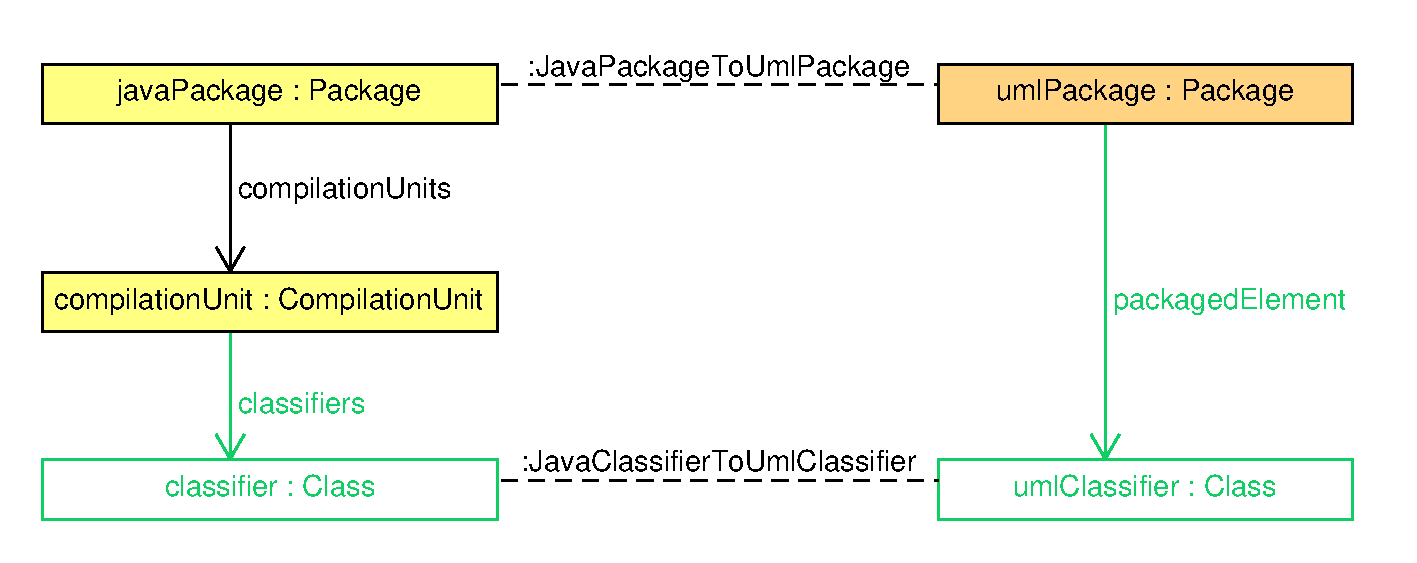
\includegraphics[width=15.5cm]{figures/tggRule_classToUmlClass.pdf}
\caption{TGG rule ClassToUmlClass}
\label{fig:classToUmlClass}
\end{figure}


\subsection{G3 - Preserving or improving performance of consistency preservation}
\label{sec:Evaluation:Results:G3}
In \autoref{fig:eval:RuntimeTrend}, the results of evaluating the prototype on \emph{HospitalToAdministration}, a case from the emoflon::IBeX tutorial \cite{emoflon_tutorial, noauthor_github_emoflon_tutorial}, using metric \emph{M3.1.1} can be seen. \textsc{VitruvTGG} performs slightly better or equal to \textsc{HiPE} up to a model size of 128 model elements (\textsc{VitruvTGG}: 116ms, \textsc{HiPE}: 115ms). From there on, \textsc{VitruvTGG} performance diverges strongly from \textsc{HiPE}'s performance.
To find out the reason for that, sub-measurements are included in \autoref{fig:eval:RuntimeTrend}. Looking at these, it stands out that coverage flattening takes up most of the total time of \textsc{VitruvTGG}, from $216$  model elements upwards it even surpasses the total execution time of \textsc{HiPE}, while the more matching-relevant measurements \emph{main green matching} and \emph{context matching} stay faster than \textsc{HiPE}, although from $4096$ model elements upwards, in tha case of \emph{main green matching}, that can be expected to change as well, but not drastically, regarding the course of the curves.
Since \emph{coverage flattening}, while being useful to find the \emph{intended} rule matches (as discussed in \cite{khelladi_detecting_complex_changes_2015}), is not necessary for the \emph{correctness} of the matching, it is of interest to look at the performance of \textsc{VitruvTGG} if coverage flattening is omitted. That is simulated by subtracting the coverage flattening time from the total change propagation time and shown in \autoref{fig:eval:RuntimeTrendWithoutCoverageFlattening}.
There it can be seen what has been suspected: While \textsc{VitruvTGG} performs better until a model size of $256$ or $512$ elements, performance diverges from there on upwards, although not as steeply as before.

To summarize, it can be said that \textbf{Q3.1} has to be answered in a differentiated way: In comparison to \textsc{HiPE}, the approach performs better or equally up to a problem size of $128$ and worse from there on upwards. So, whether \textbf{G3} has been reached depends on what problem sizes are regarded: Performance is improved or preserved and \textbf{G3} is reached for problem sizes smaller as $128$ changes in a sequence, for larger sequences, it is not and \textbf{G3} is not reached.

\begin{figure}[h!]
    \centering
    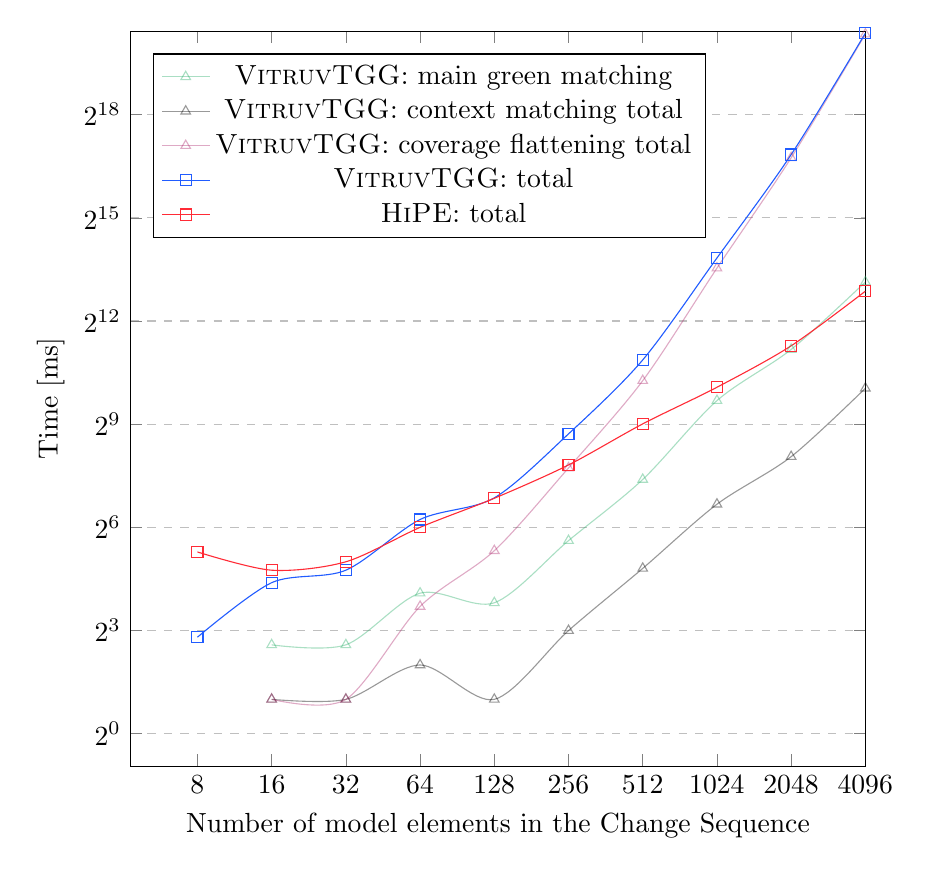
\begin{tikzpicture}
        \definecolor{myBlue}{RGB}{33,92,255}
        \definecolor{myRed}{RGB}{255,43,54}
        \definecolor{myGreen}{RGB}{42,174,105}
        \definecolor{myPurple}{RGB}{174,42,110}
        \begin{axis}[
            width=0.9\textwidth,
            height=0.9\textwidth,
            xlabel={Number of model elements in the Change Sequence},
            ylabel={Time [ms]},
            xmin=0, xmax=4096,
            ymin=0, ymax=1400000,
            xticklabels={4,8,16,32,64,128,256,512,1024,2048,4096},
            % ytick={0,10,100,1000,10000,100000},
            legend pos=north west,
            ymajorgrids=true,
            grid style=dashed,
            xmode=log,
            ymode=log,
            log basis x={2},
            log basis y={2}
        ]
        
        % VitruvTGG main green matching:
        \addplot[
            color=myGreen,
            mark=triangle,
            smooth,
            opacity=0.4,
            ]
            coordinates {
            % (8,0)(16,6)(32,4)(64,9)(128,12)(256,45)(512,145)(1024,564)(2048,2191)
            (8,0)(16,6)(32,6)(64,17)(128,14)(256,49)(512,168)(1024,823)(2048,2308)(4096,8982)
            };
        % % VitruvTGG context matching:
        \addplot[
            color=black,
            mark=triangle,
            smooth,
            opacity=0.4,
            ]
            coordinates {
            % (8,0)(16,3)(32,2)(64,4)(128,2)(256,7)(512,24)(1024,88)(2048,273)
            (8,0)(16,2)(32,2)(64,4)(128,2)(256,8)(512,28)(1024,102)(2048,266)(4096,1056)
            };
        % VitruvTGG coverage flattening:
        \addplot[
            color=myPurple,
            mark=triangle,
            smooth,
            opacity=0.4,
            ]
            coordinates {
            % (8,0)(16,2)(32,2)(64,9)(128,42)(256,189)(512,1123)(1024,8241)(2048,96266)
            (8,0)(16,2)(32,2)(64,13)(128,40)(256,212)(512,1230)(1024,11873)(2048,109831)(4096,1325673)
            };
        % VitruvTGG TOTAL:
        \addplot[
            color=myBlue,
            mark=square,
            smooth,
            ]
            coordinates {
            % (8,4)(16,25)(32,22)(64,55)(128,112)(256,386)(512,1728)(1024,10625)(2048,103277)
            (8,7)(16,21)(32,27)(64,75)(128,116)(256,421)(512,1869)(1024,14577)(2048,117092)(4096,1350937)
            };
        % HIPE TOTAL:
        \addplot[
            color=myRed,
            mark=square,
            smooth,
            ]
            coordinates {
            % (8,48)(16,18)(32,35)(64,56)(128,114)(256,209)(512,436)(1024,1138)(2048,2297)
            (8,39)(16,27)(32,32)(64,64)(128,115)(256,225)(512,515)(1024,1077)(2048,2484)(4096,7467)
            };
        \legend{
            \textsc{VitruvTGG}: main green matching,
            \textsc{VitruvTGG}: context matching total,
            \textsc{VitruvTGG}: coverage flattening total, 
            \textsc{VitruvTGG}: total, 
            \textsc{HiPE}: total
        }
            
        \end{axis}
    \end{tikzpicture}
    \caption[Runtime trend of \textsc{VitruvTGG} and \textsc{HiPE}]{Runtime trend of \textsc{VitruvTGG} and \textsc{HiPE}, median of 20 runs per measurement}
    \label{fig:eval:RuntimeTrend}
\end{figure}



\begin{figure}[h!]
    \centering
    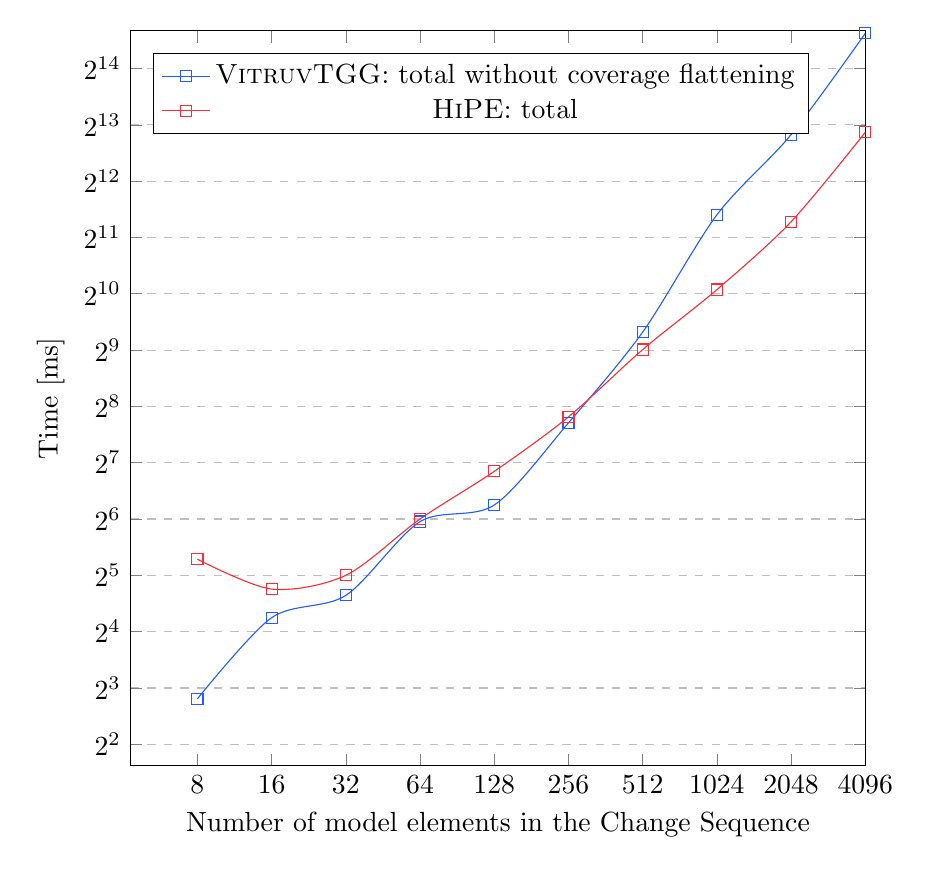
\begin{tikzpicture}
        \definecolor{myBlue}{RGB}{33,92,255}
        \definecolor{myRed}{RGB}{255,43,54}
        \begin{axis}[
            width=0.9\textwidth,
            height=0.9\textwidth,
            xlabel={Number of model elements in the Change Sequence},
            ylabel={Time [ms]},
            xmin=0, xmax=4096,
            ymin=0, ymax=26000,
            xticklabels={4,8,16,32,64,128,256,512,1024,2048,4096},
            % ytick={0,10,100,1000,10000,100000},
            legend pos=north west,
            ymajorgrids=true,
            grid style=dashed,
            xmode=log,
            ymode=log,
            log basis x={2},
            log basis y={2}
        ]
        
        % VitruvTGG TOTAL without coverage flattening:
        \addplot[
            color=myBlue,
            mark=square,
            smooth,
            ]
            coordinates {
            % (8,4)(16,25)(32,22)(64,55)(128,112)(256,386)(512,1728)(1024,10625)(2048,103277)
            (8,7)(16,19)(32,25)(64,62)(128,76)(256,209)(512,639)(1024,2704)(2048,7261)(4096,25264)
            };
        % HIPE TOTAL:
        \addplot[
            color=myRed,
            mark=square,
            smooth,
            ]
            coordinates {
            % (8,48)(16,18)(32,35)(64,56)(128,114)(256,209)(512,436)(1024,1138)(2048,2297)
            (8,39)(16,27)(32,32)(64,64)(128,115)(256,225)(512,515)(1024,1077)(2048,2484)(4096,7467)
            };
        \legend{
            \textsc{VitruvTGG}: total without coverage flattening, 
            \textsc{HiPE}: total
        }
        \end{axis}
    \end{tikzpicture}
    \caption[Runtime trend of \textsc{VitruvTGG} without coverage flattening and \textsc{HiPE}]{Runtime trend of \textsc{VitruvTGG} without coverage flattening and \textsc{HiPE}, median of 20 runs per measurement}
    \label{fig:eval:RuntimeTrendWithoutCoverageFlattening}
\end{figure}
        % Template:
        %(8,)(16,)(32,)(64,)(128,)(256,)(512,)(1024,)(2048,)
